\documentclass[border=12pt]{standalone}
\def\pgfsysdriver{pgfsys-dvisvgm.def}
\usepackage[dvisvgm]{xcolor}
\usepackage{xeCJK}
\setCJKmainfont{HaranoAjiGothic-Regular.otf}[BoldFont=HaranoAjiGothic-Bold.otf]
\setCJKsansfont{HaranoAjiGothic-Regular.otf}[BoldFont=HaranoAjiGothic-Bold.otf]
\usepackage{amsmath,amssymb,tikz,lmodern}
\usetikzlibrary{arrows.meta,positioning,calc,fit,backgrounds}
\renewcommand{\familydefault}{\sfdefault}
\definecolor{ink}{HTML}{25322F}
\definecolor{green}{HTML}{246657}
\definecolor{tint}{HTML}{EEF4F0}
\definecolor{soft}{HTML}{C6D2CC}
\definecolor{muted}{HTML}{52615B}
\newif\ifJapanese
\newcommand{\Tx}[2]{\ifJapanese #1\else #2\fi}
\newcommand{\Eff}{\overline{\operatorname{Eff}}}
\newcommand{\heading}[3]{{\color{green}\bfseries #1\quad\Tx{#2}{#3}}\\[5pt]}
% A white rectangle makes the complete citation label clickable, including spaces.
\newcommand{\refurl}[2]{\special{dvisvgm:raw <a xlink:href="#1" target="_blank" rel="noopener noreferrer">}{\setlength{\fboxsep}{0pt}\colorbox{white}{\color{green}\underline{\strut #2}}}\special{dvisvgm:raw </a>}}
\tikzset{
 card/.style={draw=soft,fill=white,rounded corners=2pt,align=left,text=ink,font=\fontsize{10.5}{14}\selectfont,inner xsep=12pt,inner ysep=10pt,text width=16cm},
 half/.style={card,text width=7.1cm,minimum height=2.05cm},
 result/.style={draw=green,fill=tint,line width=.9pt},
 reason/.style={align=left,text=muted,font=\fontsize{9}{12}\selectfont,inner sep=0pt,text width=14.3cm},
 branchreason/.style={reason,text width=6.4cm},
 edge/.style={-{Stealth[length=2.4mm]},draw=green,line width=1pt},
 wire/.style={draw=green,line width=1pt},
}
% Keep the arrow in a dedicated left gutter; explanations never cover it.
\newcommand{\flow}[3]{
 \coordinate (#2-from) at ($(#1.south)+(-7.7,0)$);
 \coordinate (#2-to) at ($(#2.north)+(-7.7,0)$);
 \draw[edge] (#2-from)--(#2-to);
 \node[reason,anchor=west] (#2-reason) at ($(#2-from)!.5!(#2-to)+(.55,0)$) {#3};
}

\newcommand{\RA}[1]{\refurl{\sourceRA}{#1}}
\newcommand{\OI}[1]{\refurl{\sourceOI}{#1}}
\newcommand{\FF}[1]{\refurl{\sourceFF}{#1}}
\newcommand{\FFcor}[1]{\refurl{\sourceFFcor}{#1}}
\newcommand{\BBT}[1]{\refurl{\sourceBBT}{#1}}
\newcommand{\FG}[1]{\refurl{\sourceFG}{#1}}
\newcommand{\CP}[1]{\refurl{\sourceCP}{#1}}
\newcommand{\BDPP}[1]{\refurl{\sourceBDPP}{#1}}
\newcommand{\pe}{\mathrel{\geq_{\mathrm{pe}}}}
\newcommand{\rowflow}[3]{
 \coordinate (#2-a) at ($(#1.south)+(-3.45,0)$);
 \coordinate (#2-b) at ($(#2.north)+(-3.45,0)$);
 \draw[edge] (#2-a)--(#2-b);
 \node[branchreason,anchor=west] at ($(#2-a)!.5!(#2-b)+(.45,0)$) {#3};
}

\newcommand{\sourceRA}{https://github.com/openai/math/blob/fd4aeeb2ee4fc729c18d98444fed42fd0529eeeb/preprints/The-reverse-logarithmic-Kodaira-inequality-and-additivity-September-26-2026/paper.pdf}
\newcommand{\sourceOI}{https://github.com/openai/math/blob/fd4aeeb2ee4fc729c18d98444fed42fd0529eeeb/preprints/Orbifold-and-logarithmic-Iitaka-subadditivity-September-26-2026/paper.pdf}
\newcommand{\sourceFF}{https://www.math.kyoto-u.ac.jp/~fujino/vmhs-sp108.pdf}
\newcommand{\sourceFFcor}{https://www.math.kyoto-u.ac.jp/~fujino/fujino-fujisawa-memo2.pdf}
\newcommand{\sourceBBT}{https://arxiv.org/pdf/1811.12230v3}
\newcommand{\sourceFG}{https://www.numdam.org/item/10.5802/aif.2894.pdf}
\newcommand{\sourceCP}{https://arxiv.org/pdf/1508.02456v4}
\newcommand{\sourceBDPP}{https://arxiv.org/pdf/math/0405285v1}
\Japanesetrue
\begin{document}
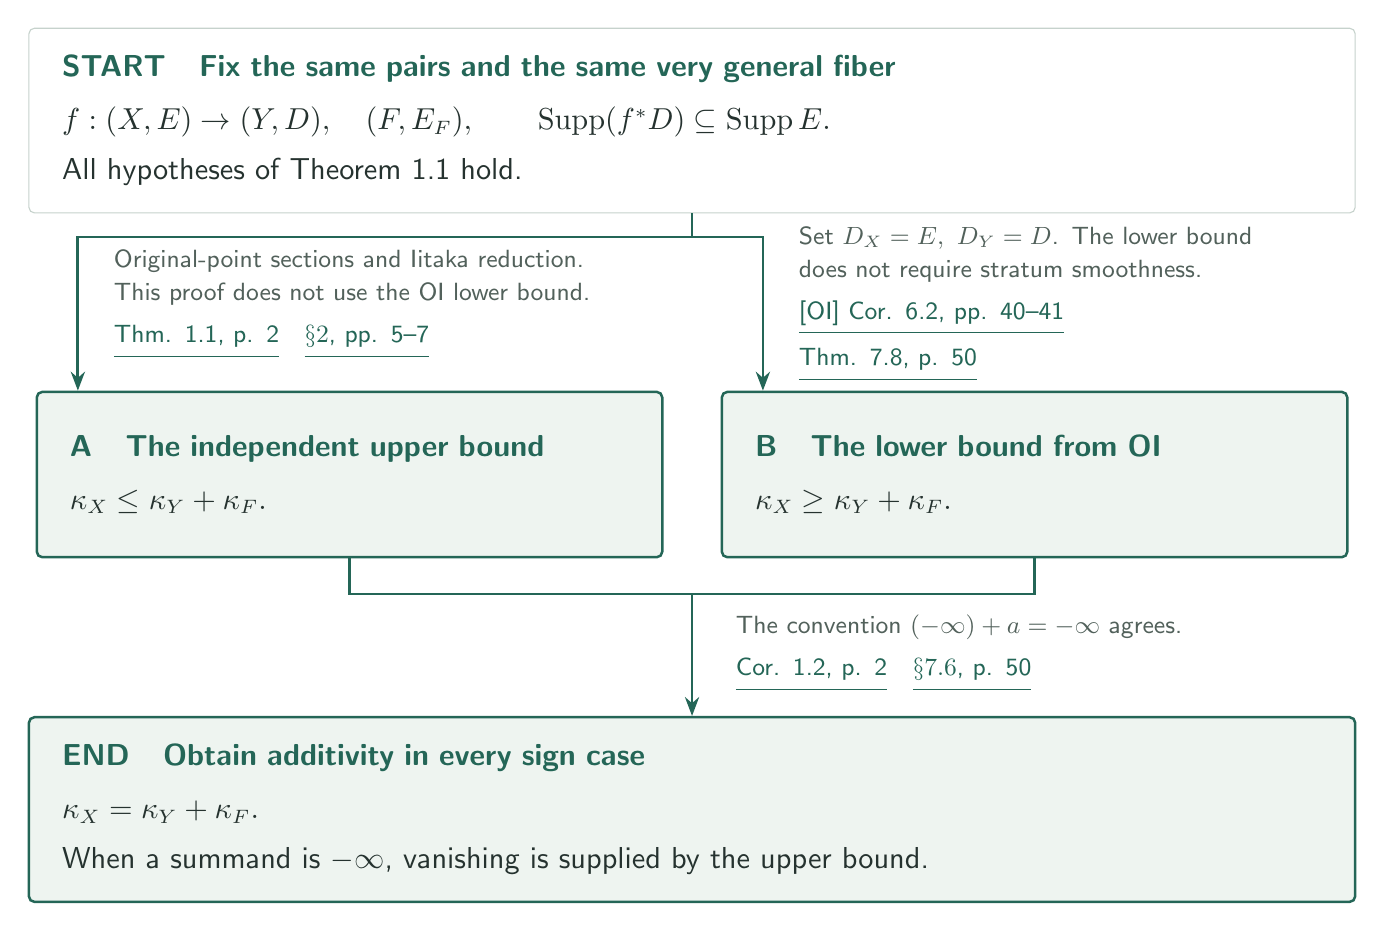
\begin{tikzpicture}
\node[card] (start) {\heading{START}{同じ対と非常に一般のファイバーを固定する}{Fix the same pairs and the same very general fiber}
$f:(X,E)\to(Y,D),\quad(F,E_F),\qquad\operatorname{Supp}(f^*D)\subseteq\operatorname{Supp}E.$\\[4pt]
\Tx{Theorem 1.1の全仮定を満たす。}{All hypotheses of Theorem 1.1 hold.}};
\node[half,result,below=2.25cm of start.south,anchor=north,xshift=-4.35cm,minimum height=2.1cm] (upper) {\heading{A}{本稿の独立した上界}{The independent upper bound}
$\kappa_X\leq\kappa_Y+\kappa_F.$};
\node[half,result,below=2.25cm of start.south,anchor=north,xshift=4.35cm,minimum height=2.1cm] (lower) {\heading{B}{OIによる下界}{The lower bound from OI}
$\kappa_X\geq\kappa_Y+\kappa_F.$};
\draw[wire] (start.south)--++(0,-.3) coordinate (fork);
\draw[edge] (fork)-|($(upper.north)+(-3.45,0)$);
\draw[edge] (fork)-|($(lower.north)+(-3.45,0)$);
\node[branchreason,anchor=west] at ($(upper.north)+(-3,1.1)$) {\Tx{元の点を保つ切断構成と飯高帰着。\\OIの下界を用いない。}{Original-point sections and Iitaka reduction.\\This proof does not use the OI lower bound.}\\[3pt]\RA{Thm. 1.1, p. 2}\quad\RA{$\S2$, pp. 5--7}};
\node[branchreason,anchor=west] at ($(lower.north)+(-3,1.1)$) {\Tx{$D_X=E,\ D_Y=D$ とする。\\下界はstratumの滑らかさを要求しない。}{Set $D_X=E,\ D_Y=D$. The lower bound\\does not require stratum smoothness.}\\[3pt]\OI{[OI] Cor. 6.2, pp. 40--41}\\[2pt]\RA{Thm. 7.8, p. 50}};
\node[card,result,below=2cm of upper.south,anchor=north,xshift=4.35cm] (end) {\heading{END}{全ての符号の場合で加法性を得る}{Obtain additivity in every sign case}
$\kappa_X=\kappa_Y+\kappa_F.$\\[4pt]
\Tx{右辺に $-\infty$ が現れるときの消滅は、上界が与える。}{When a summand is $-\infty$, vanishing is supplied by the upper bound.}};
\coordinate (join) at ($(end.north)+(0,1.55)$);
\draw[wire] (upper.south)|-(join);
\draw[wire] (lower.south)|-(join);
\draw[edge] (join)--($(end.north)+(0,0)$);
\node[reason,text width=7cm,anchor=west] at ($(end.north)+(.55,.8)$) {\Tx{$(-\infty)+a=-\infty$ の規約も一致する。}{The convention $(-\infty)+a=-\infty$ agrees.}\\[3pt]\RA{Cor. 1.2, p. 2}\quad\RA{$\S7.6$, p. 50}};
\end{tikzpicture}

\end{document}
